\documentclass{article}

\usepackage{graphicx}
\usepackage[utf8]{inputenc}
\usepackage[russian]{babel}
\usepackage{mathtools}
\title{1.1}
\author{svbor2000 }
\date{April 2022}

\begin{document}
\begin{center}
"Теоретические модели вычислений" \\
Бородин Сергей Владимирович А-13а-19
\end{center}
\vspace{6em}




\newpage
\textbf{Задание 1. Построить конечный автомат, распознающий язык}\\
1.1\\
L = \{\omega \in \{a, b, c\}^* \mid |\omega|_c = 1\}\\
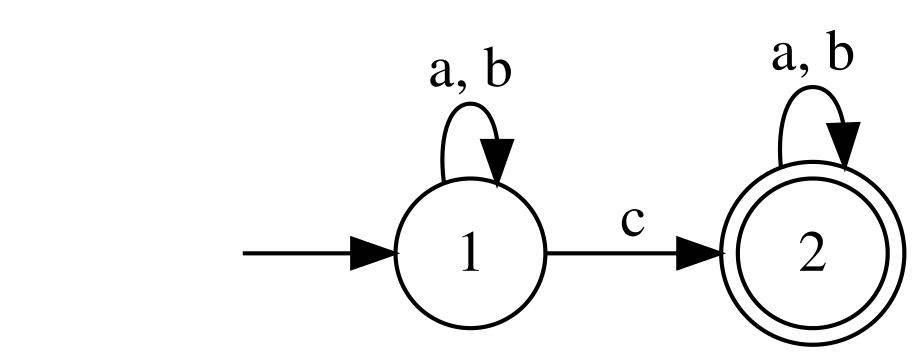
\includegraphics {1_1.png}\\
1.2\\
L = \{\omega \in \{a, b\}^* \mid |\omega|_a \leq 2, |\omega|_b \geq 2\}\\

\begin{tabular} {|c |c |c|}
\hline
 & a & b \\
\hline
\(q_1,q_4\) & \(q_2,q_4\) & \(q_1,q_5\) \\
\hline
\(q_1,q_5\) & \(q_2,q_5\) & \(q_1,q_6\) \\
\hline
\(q_1,q_6\) & \(q_2,q_6\) & \(q_1,q_6\) \\
\hline
\(q_2,q_4\) & \(q_3,q_4\) & \(q_2,q_5\) \\
\hline
\(q_2,q_5\) & \(q_3,q_5\) & \(q_2,q_6\) \\
\hline
\(q_2,q_6\) & \(q_3,q_6\) & \(q_2,q_6\) \\
\hline
\(q_3,q_4\) & \(\emptyset\) & \(q_3,q_5\) \\
\hline
\(q_3,q_5\) & \(\emptyset\) & \(q_3,q_6\) \\
\hline
\(q_3,q_6\) & \(\emptyset\) & \(q_3,q_6\) \\
\hline
\end{tabular}\\
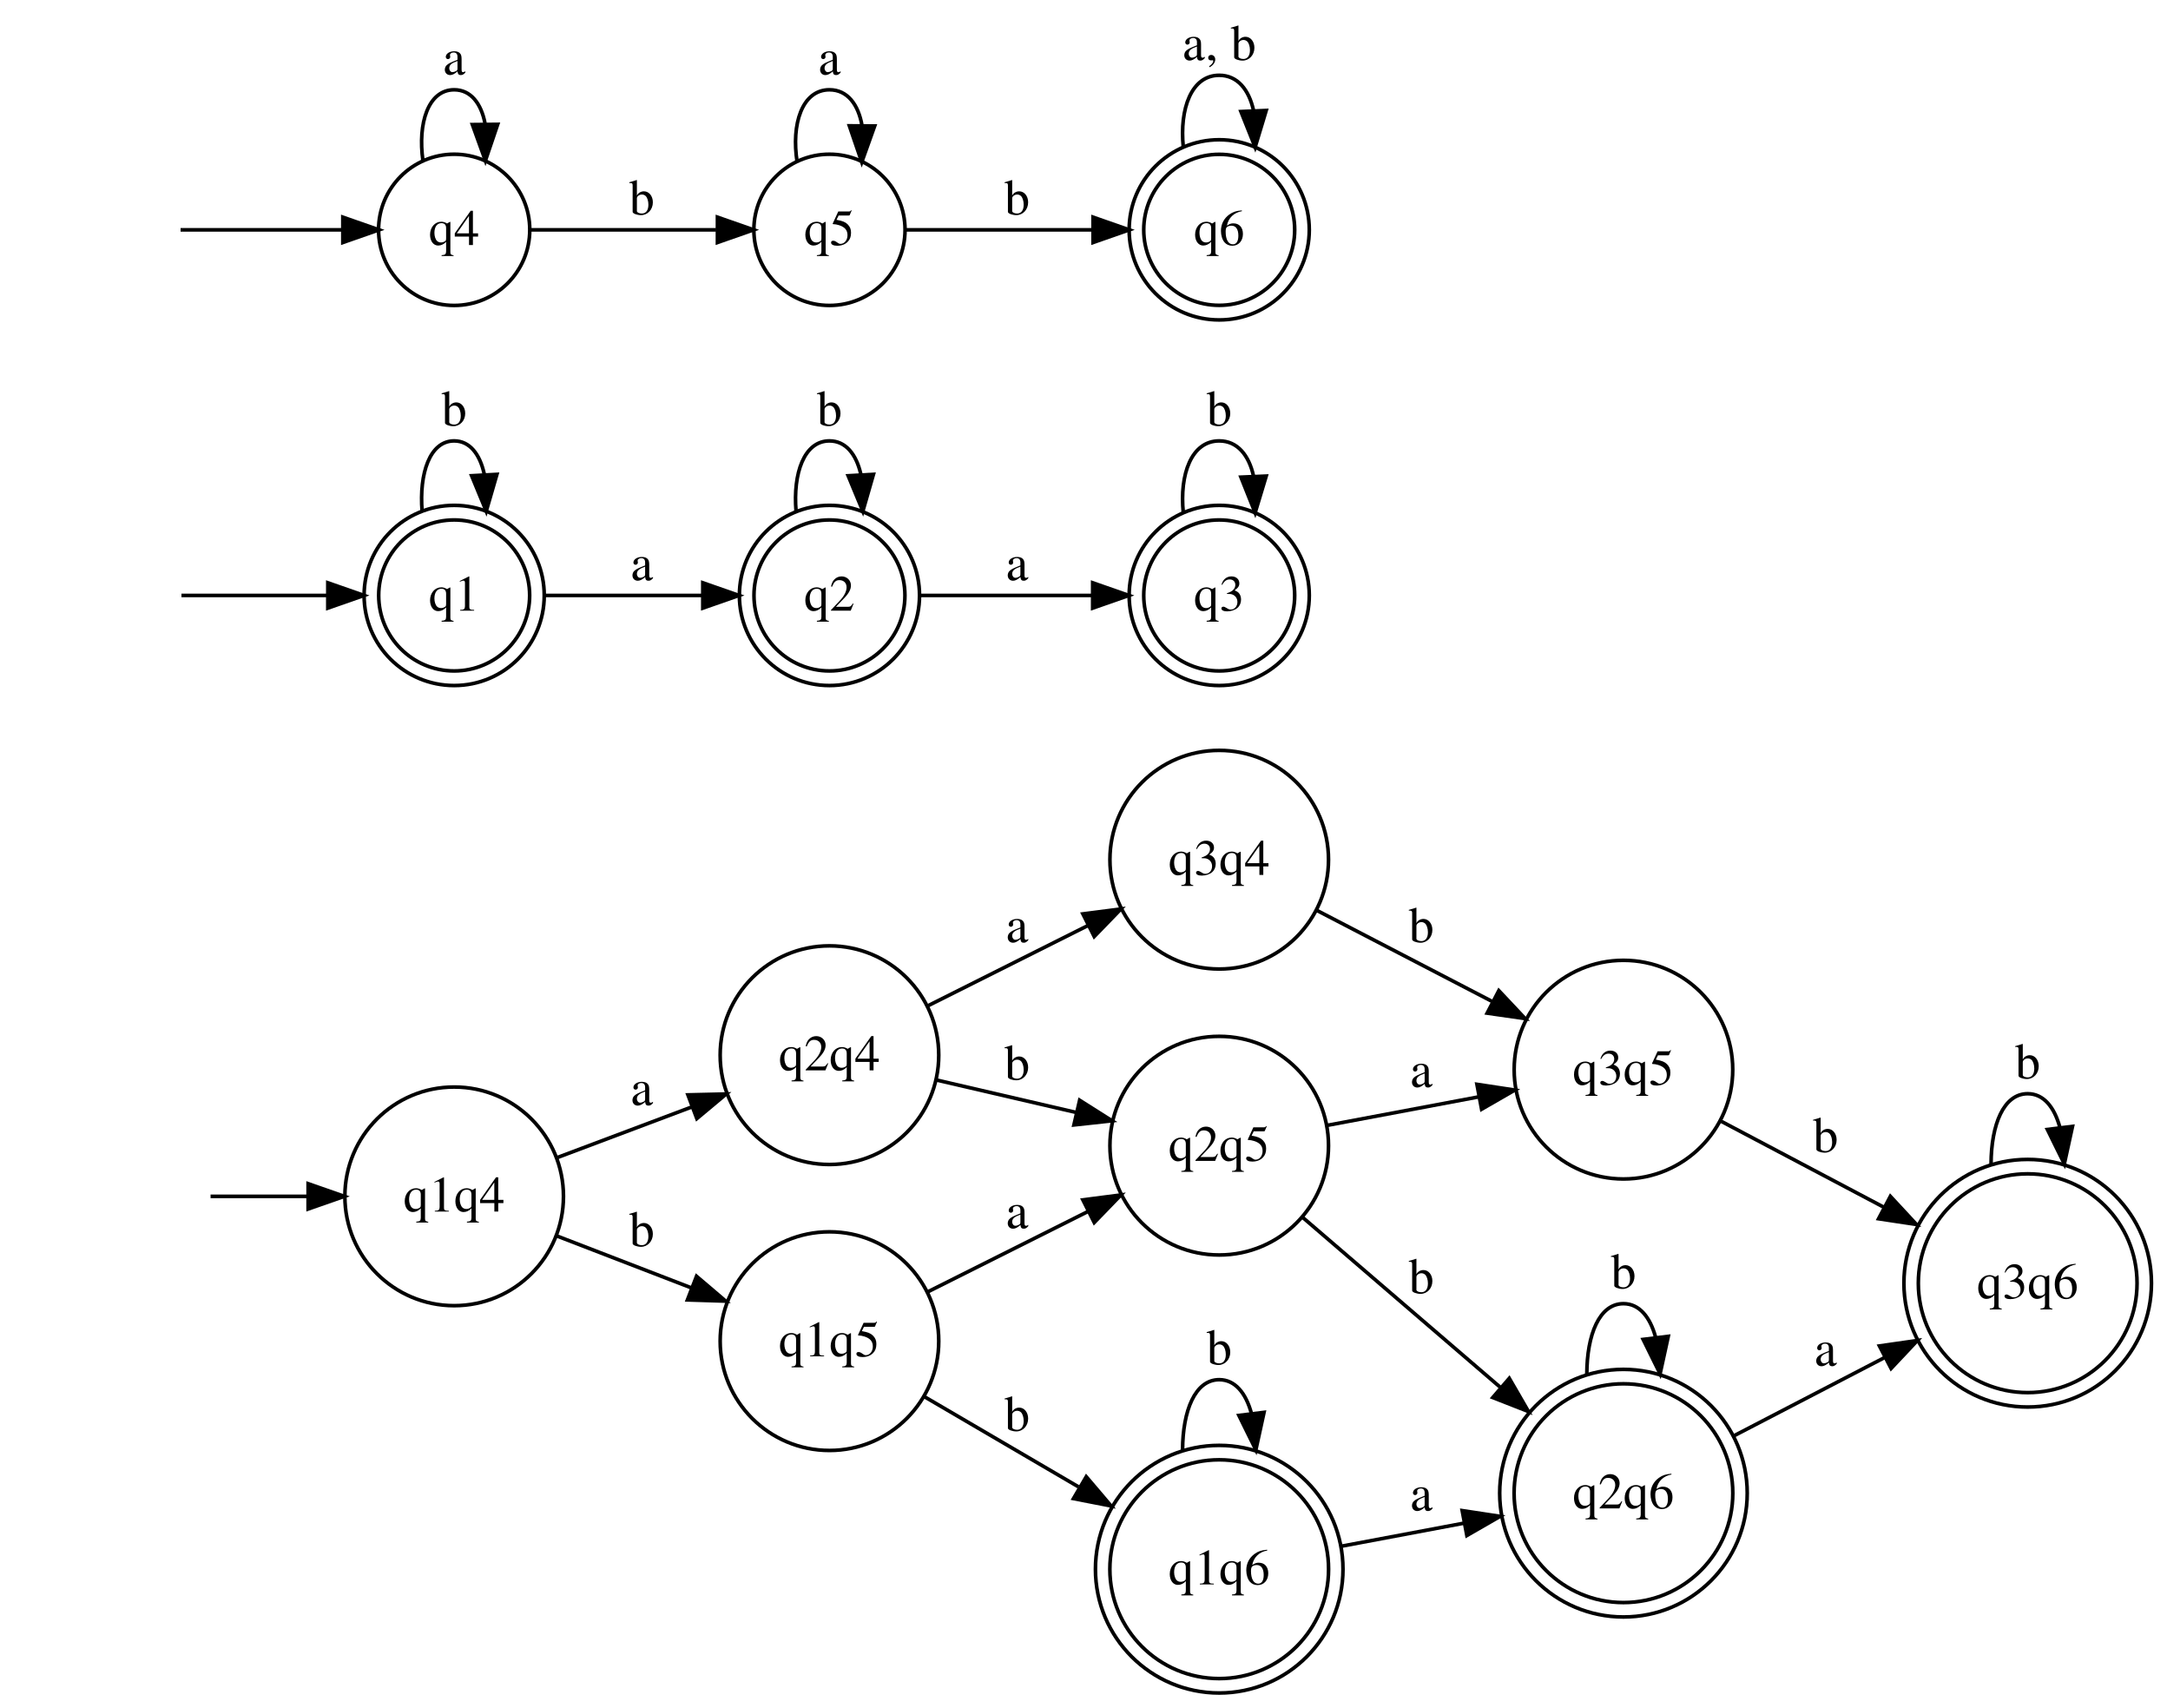
\includegraphics [scale=0.2]{1_2.png}\\
1.3\\
L = \{\omega \in \{a, b\}^* \mid |\omega|_a \neq  |\omega|_b\}\\
\text{Язык нельзя описать с помощью ДКА, так как нелюхлдимо запоминать кол-во символов хотябы  одного типа, а ДКА этого сделать не может}\\
1.4\\
L = \{\omega \in \{a, b\}^* \mid  \omega\omega =  \omega\omega\omega\}\\
\text{Содержит пустые слова}\\
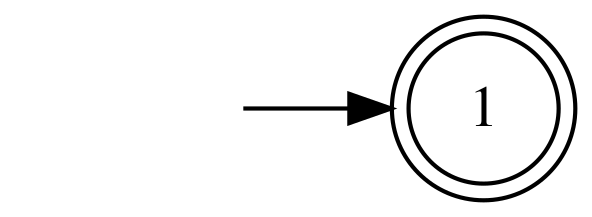
\includegraphics [scale=0.7]{1_4.png}\\
\textbf{Задание 2. Построить конечный автомат,используя прямое произведени}\\
2.1\\
L = \{\omega \in \{a, b\} \mid |\omega|_a \geq 2 \wedge |\omega|_b \geq 2\}\\
\begin{tabular} {|c |c |c|}
\hline
 & a & b \\
\hline
\(q_1,q_4\) & \(q_2,q_4\) & \(q_1,q_5\) \\
\hline
\(q_1,q_5\) & \(q_2,q_5\) & \(q_1,q_6\) \\
\hline
\(q_1,q_6\) & \(q_2,q_6\) & \(q_1,q_6\) \\
\hline
\(q_2,q_4\) & \(q_3,q_4\) & \(q_2,q_5\) \\
\hline
\(q_2,q_5\) & \(q_3,q_5\) & \(q_2,q_6\) \\
\hline
\(q_2,q_6\) & \(q_3,q_6\) & \(q_2,q_6\) \\
\hline
\(q_3,q_4\) & \(q_3,q_4\) & \(q_3,q_5\) \\
\hline
\(q_3,q_5\) & \(q_3,q_5\) & \(q_3,q_6\) \\
\hline
\(q_3,q_6\) & \(q_3,q_6\) & \(q_3,q_6\) \\
\hline
\end{tabular}\\
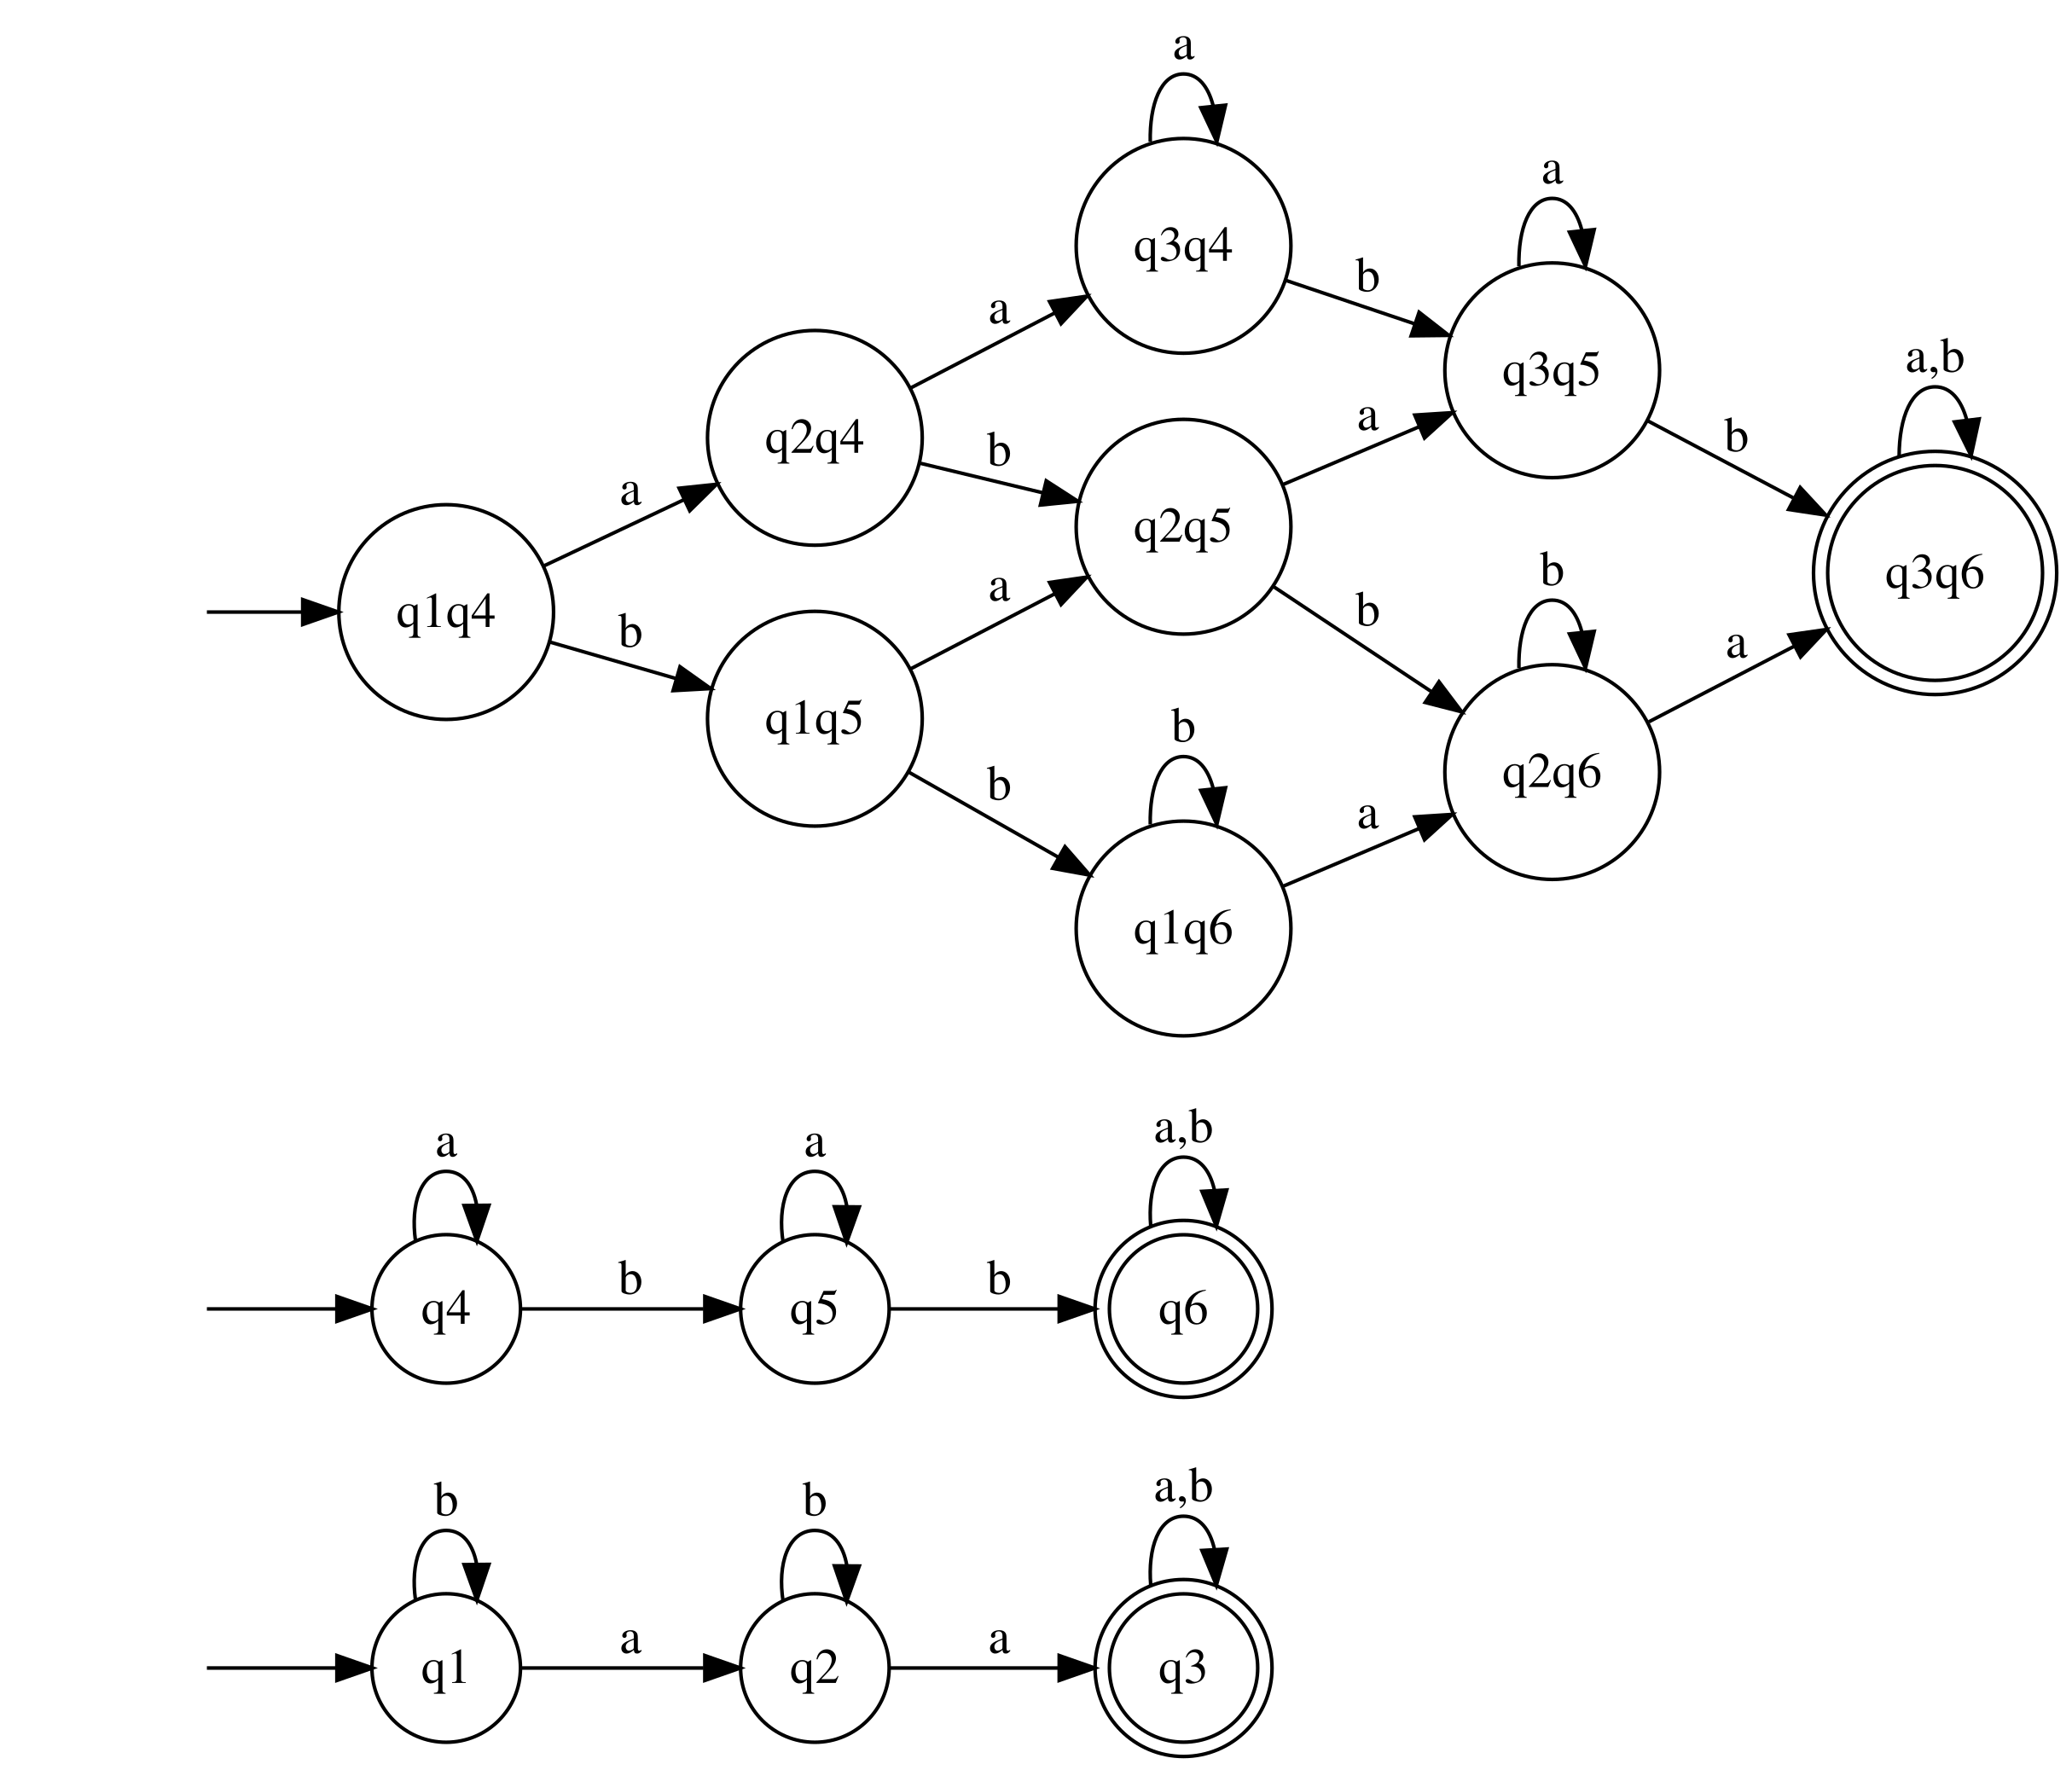
\includegraphics [scale=0.7]{2_1.png}\\\\
2.2\\
L = \{\omega \in \{a, b\}^* \mid |\omega| \geq 3 \wedge |\omega| \text{ нечетное}\}\\
\\
\begin{tabular} {|c |c |c|}
\hline
 & a & b \\
\hline
\(q_1,q_5\) & \(q_2,g_6\) & \(q_2,g_6\) \\
\hline
\(q_1,q_6\) & \(q_2,g_5\) & \(q_2,g_5\) \\
\hline
\(q_2,q_5\) & \(q_3,g_6\) & \(q_3,g_6\) \\
\hline
\(q_2,q_6\) & \(q_3,g_5\) & \(q_3,g_5\) \\
\hline
\(q_3,q_5\) & \(q_4,g_6\) & \(q_4,g_6\) \\
\hline
\(q_3,q_6\) & \(q_4,g_5\) & \(q_4,g_5\) \\
\hline
\(q_4,q_5\) & \(q_4,g_6\) & \(q_4,g_6\) \\
\hline
\(q_4,q_6\) & \(q_4,g_5\) & \(q_4,g_5\) \\
\hline
\end{tabular}\\
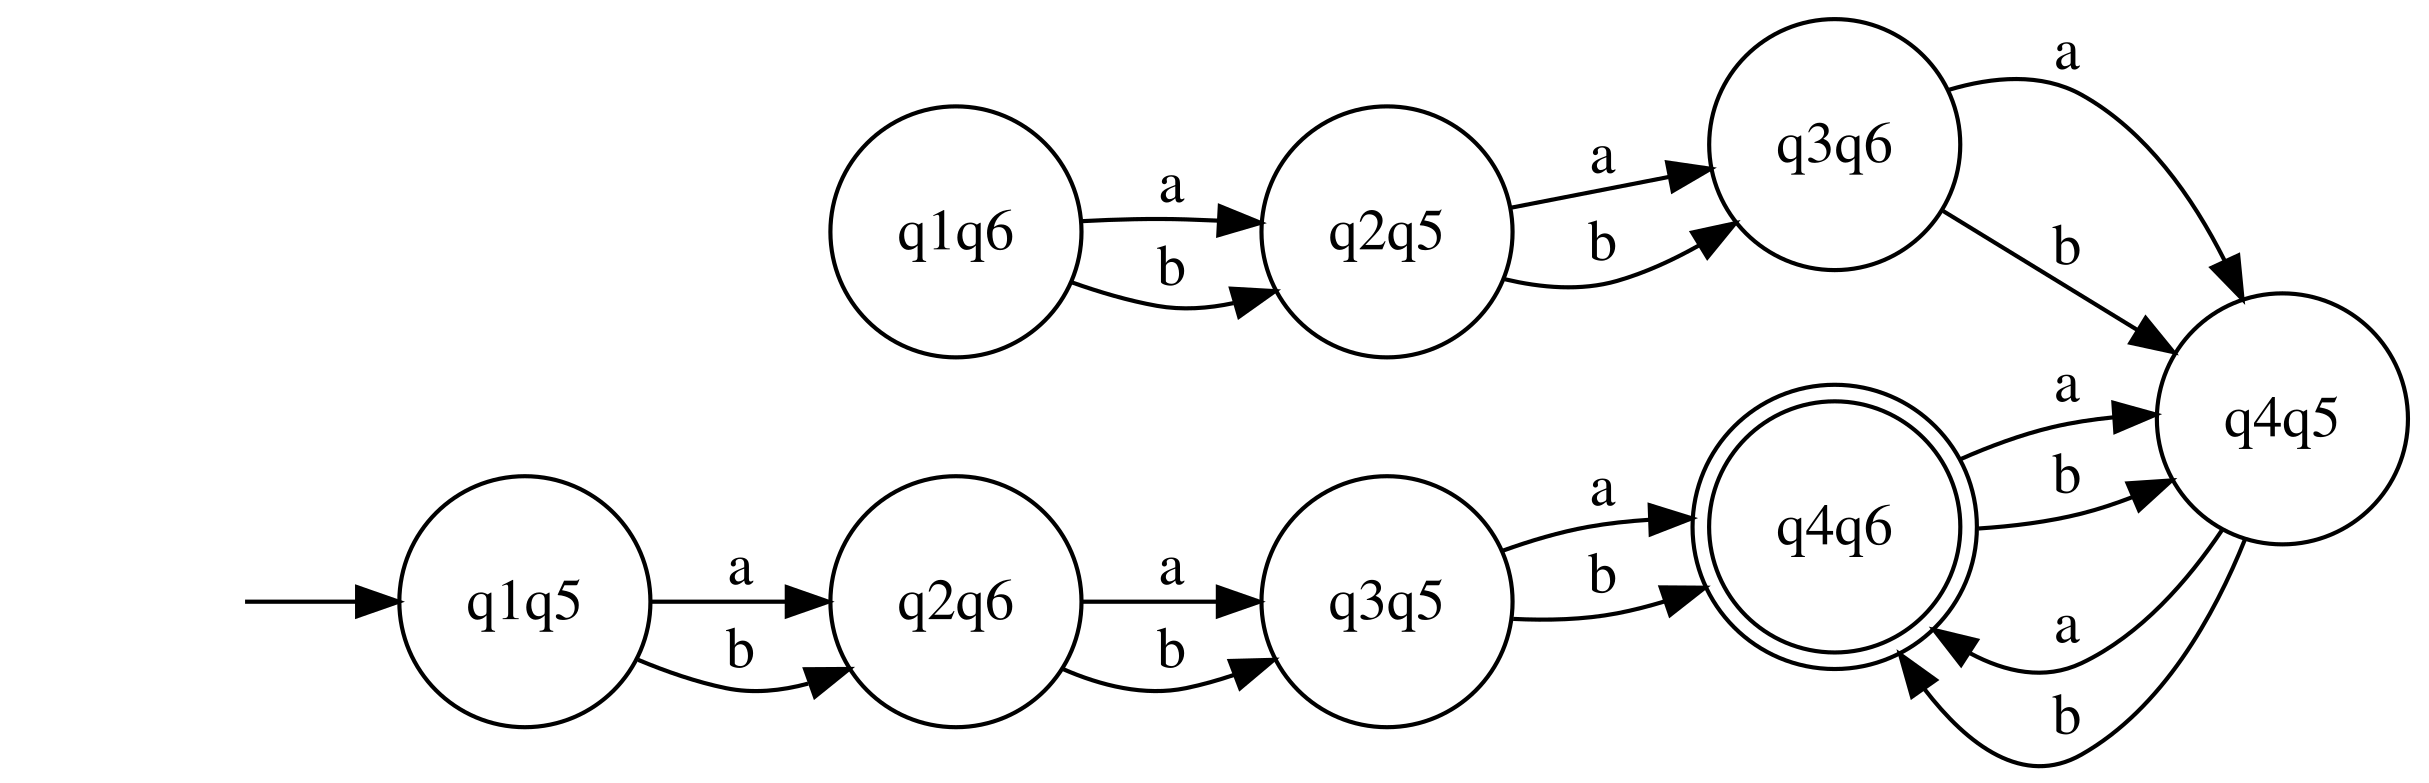
\includegraphics [scale=0.7]{2.2_pred_dot.png}\\
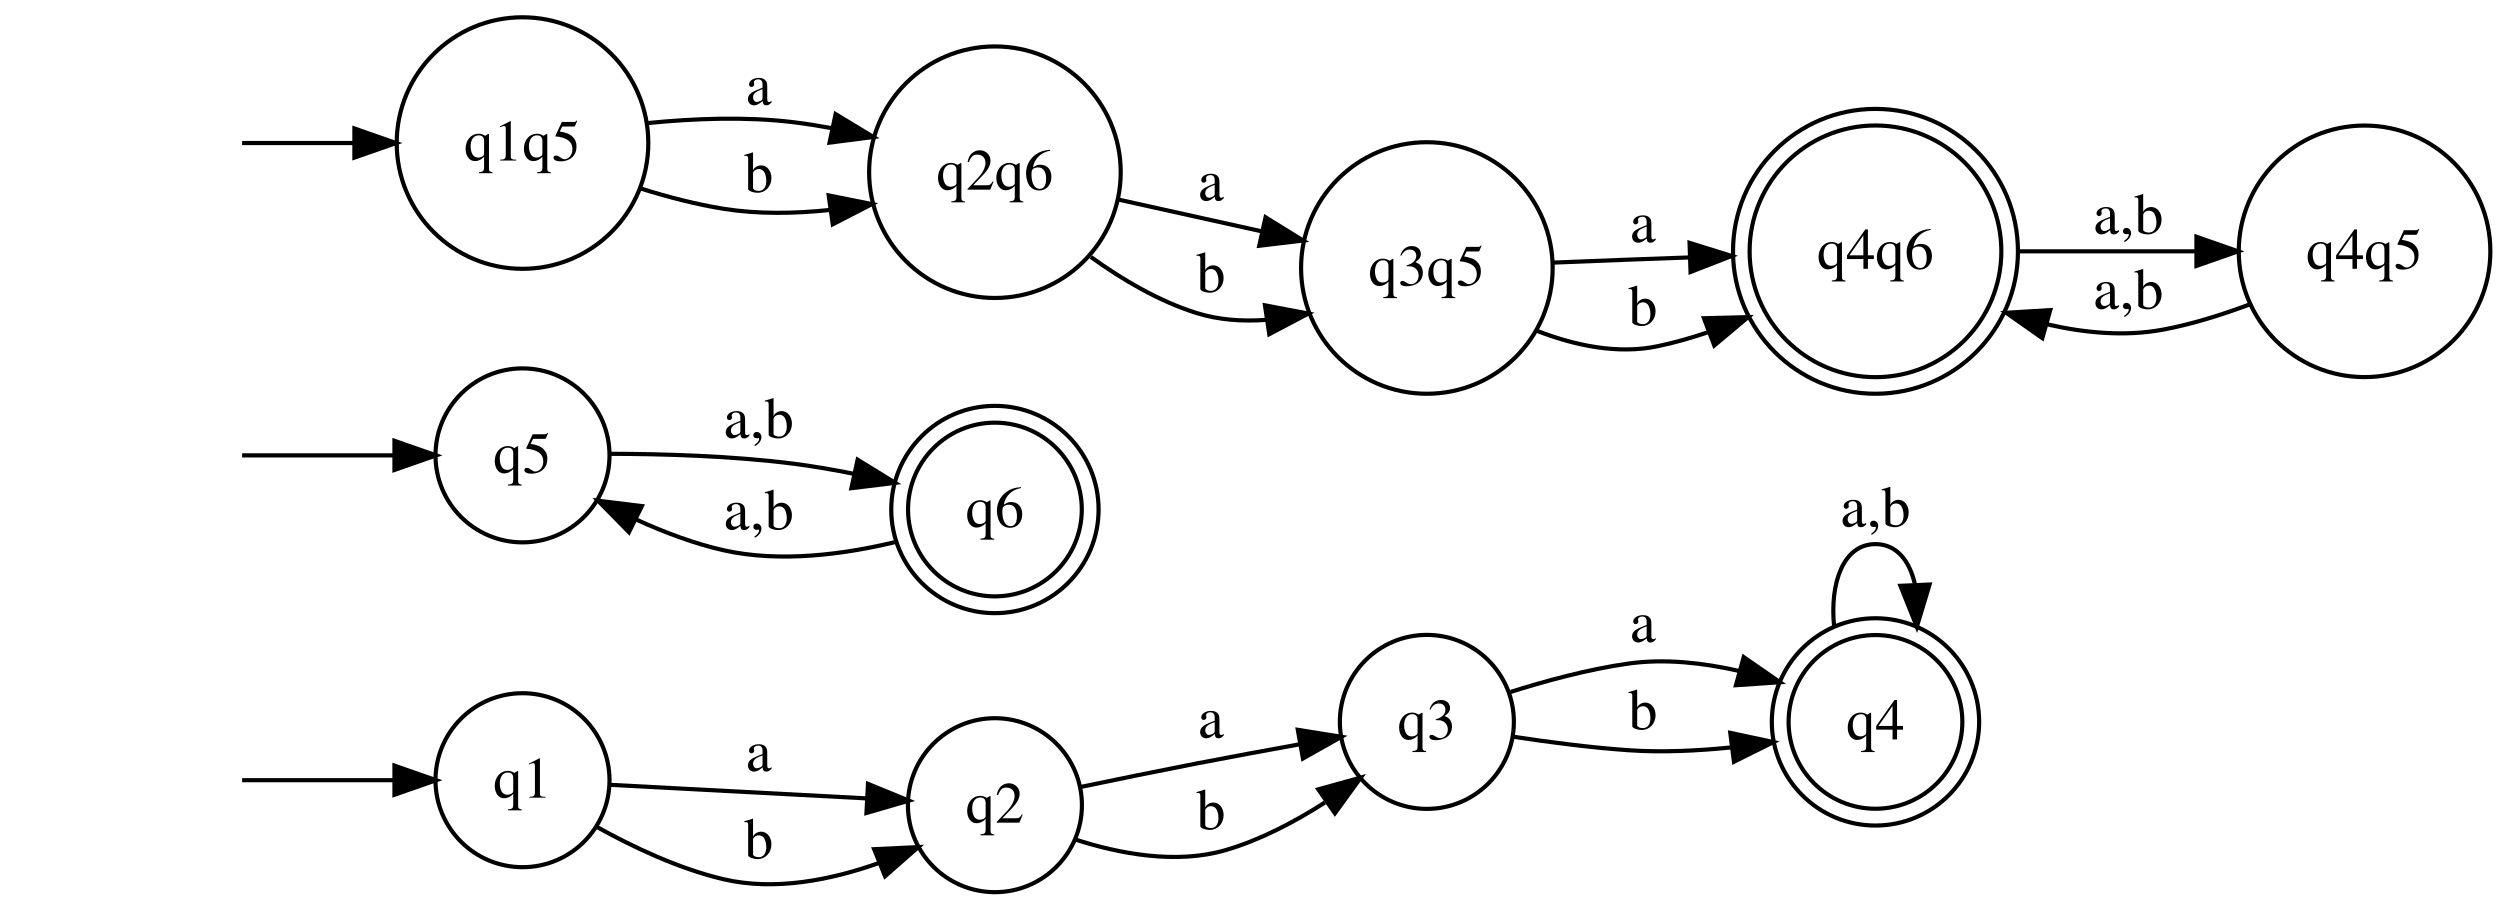
\includegraphics [scale=0.7]{2_2.png}\\\\

2.3\\
L = \{\omega \in \{a, b\}^* \mid |\omega|_a \text{ четное} \wedge |\omega|_b \text{ кратно 3}\}\\
\\
\begin{tabular} {|c |c |c|}
\hline
 & a & b \\
\hline
\(q_1,q_4\) & \(q_1,g_5\) & \(q_2,g_4\) \\
\hline
\(q_1,q_5\) & \(q_1,g_4) & \(q_2,g_5\) \\
\hline
\(q_2,q_4\) & \(q_2,g_5\) & \(q_3,g_4\) \\
\hline
\(q_2,q_5\) & \(q_2,g_4\) & \(q_3,g_5\) \\
\hline
\(q_3,q_4\) & \(q_3,g_5\) & \(q_1,g_4\) \\
\hline
\(q_3,q_5\) & \(q_3,g_4\) & \(q_1,g_5\) \\
\hline
\end{tabular}\\
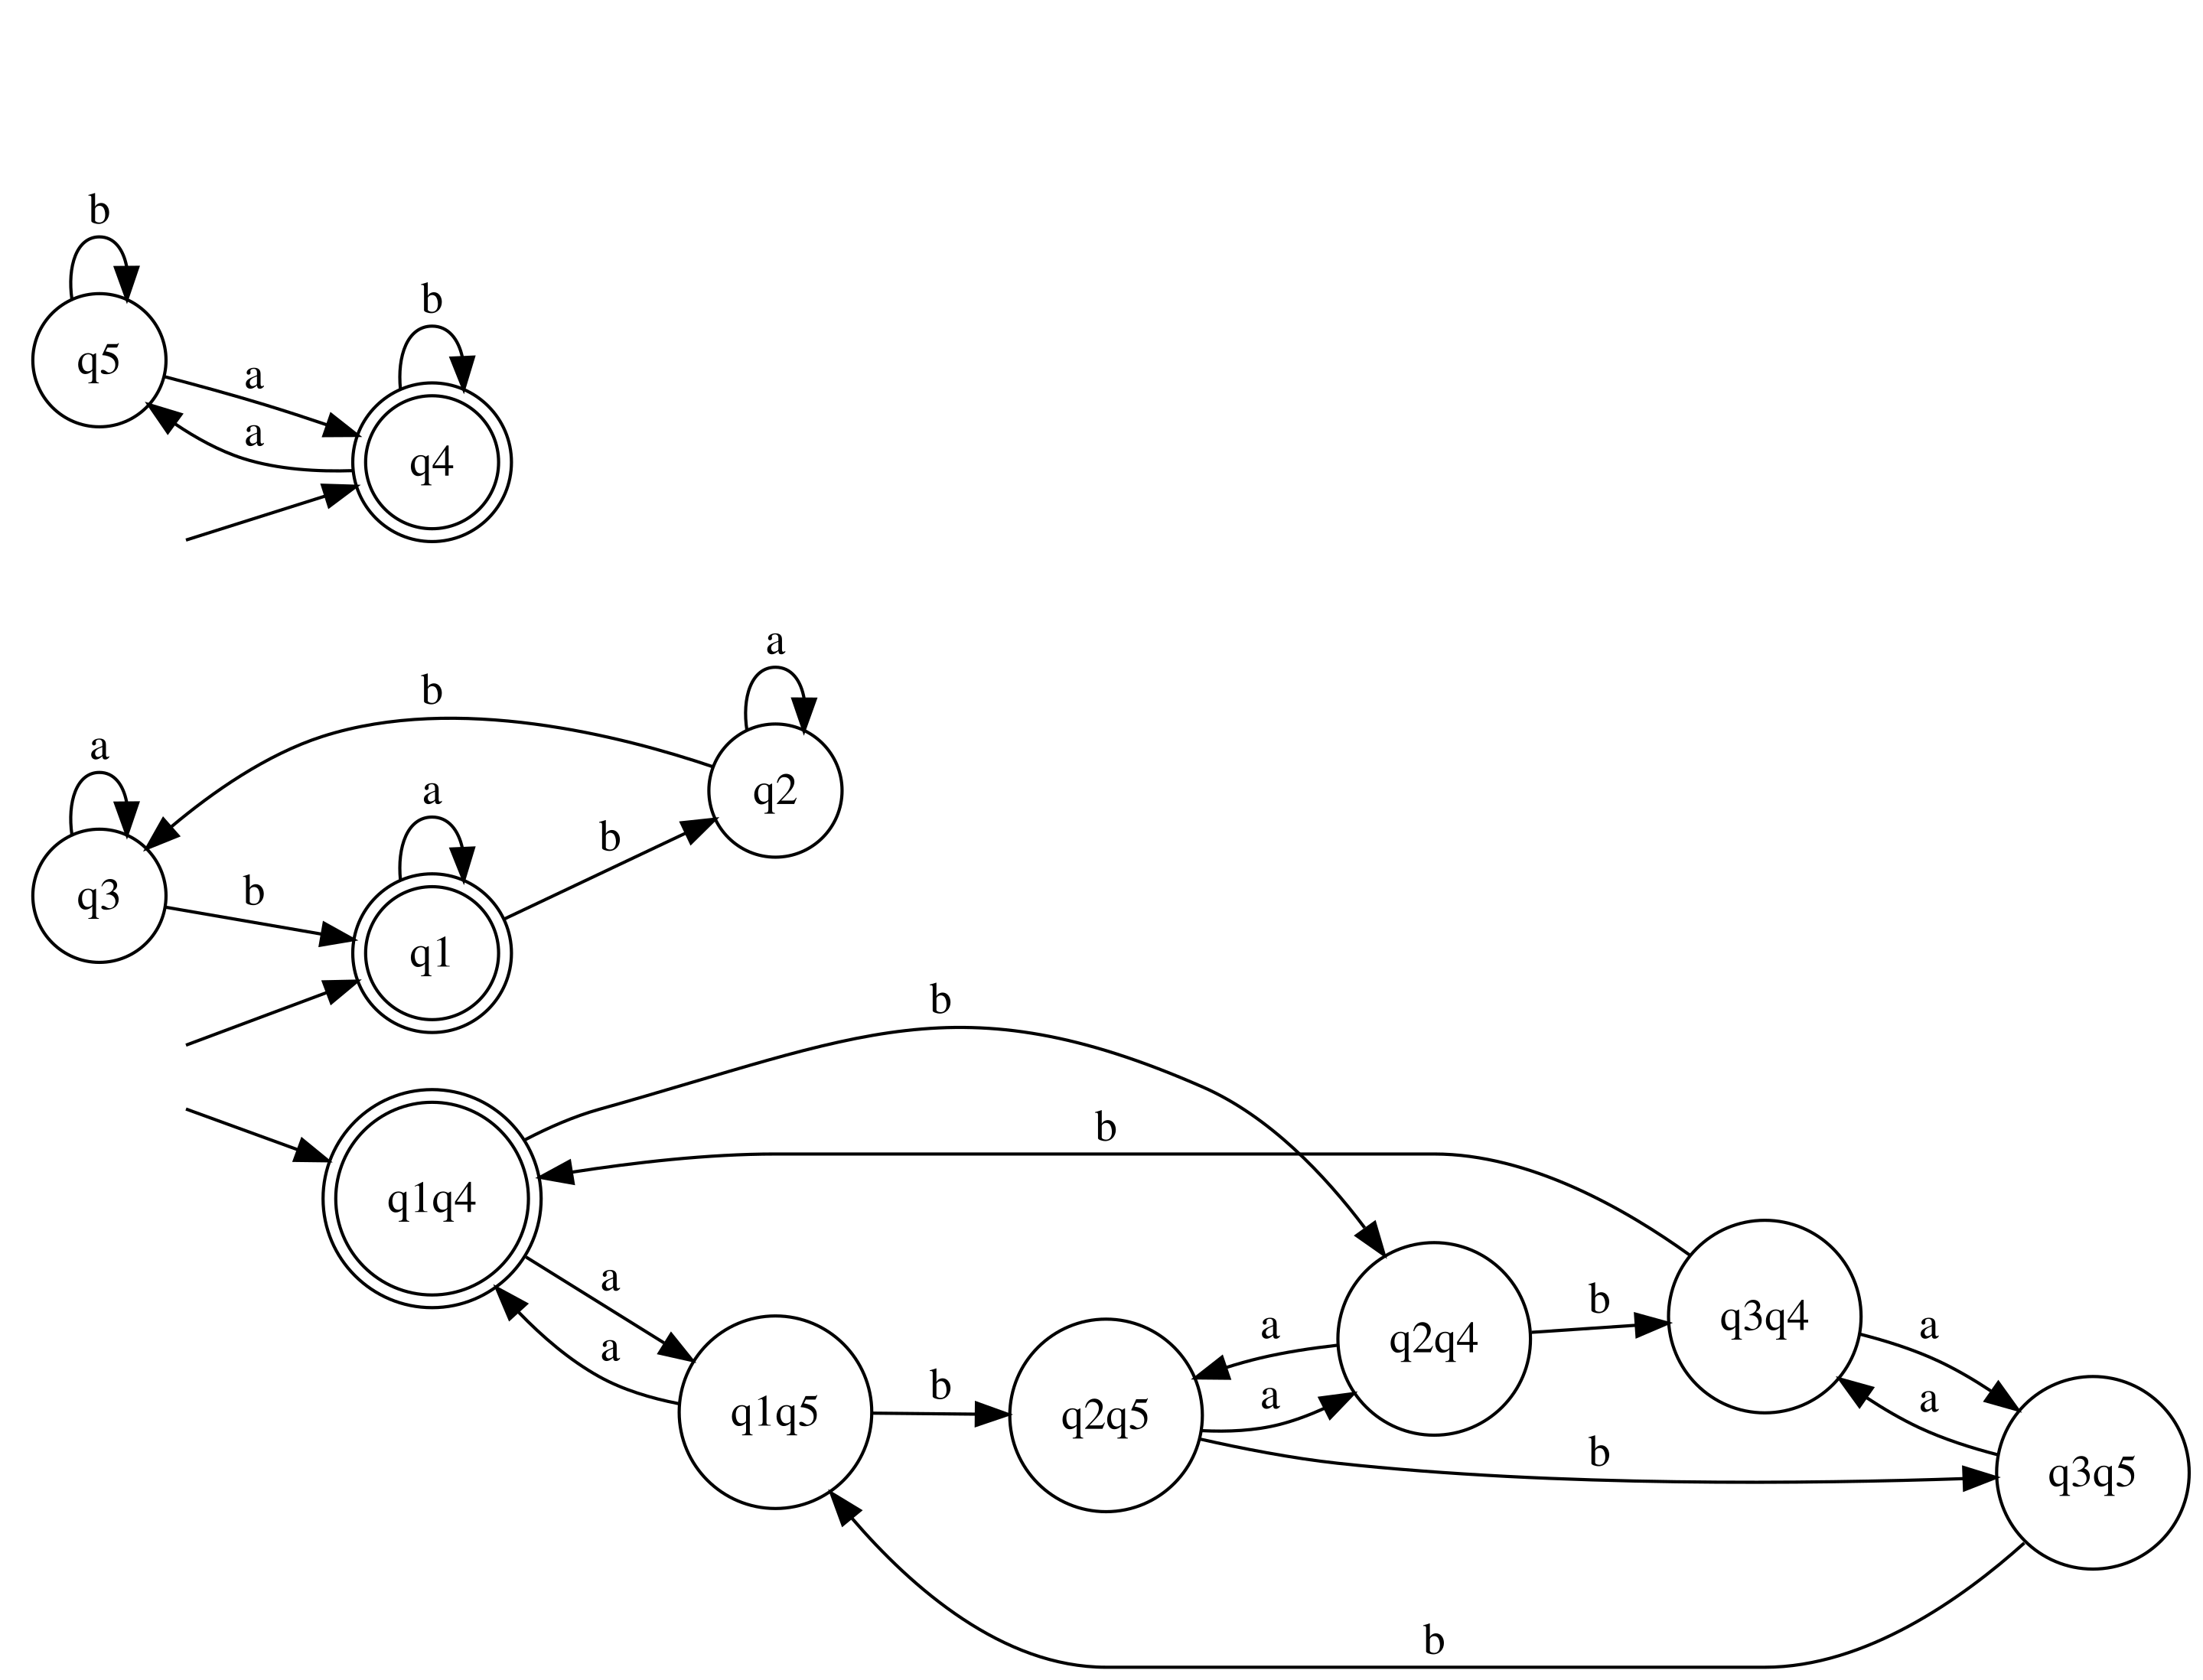
\includegraphics [scale=0.7]{2_3.png}\\\\
2.4\\
L_4 = \bar{L_3} \\
T_4 = Q_3 \ T_3 = {q_1q_4, q_1q_5, q_2q_4, q_2q_5, q_3q_4, q_3q_5}\\
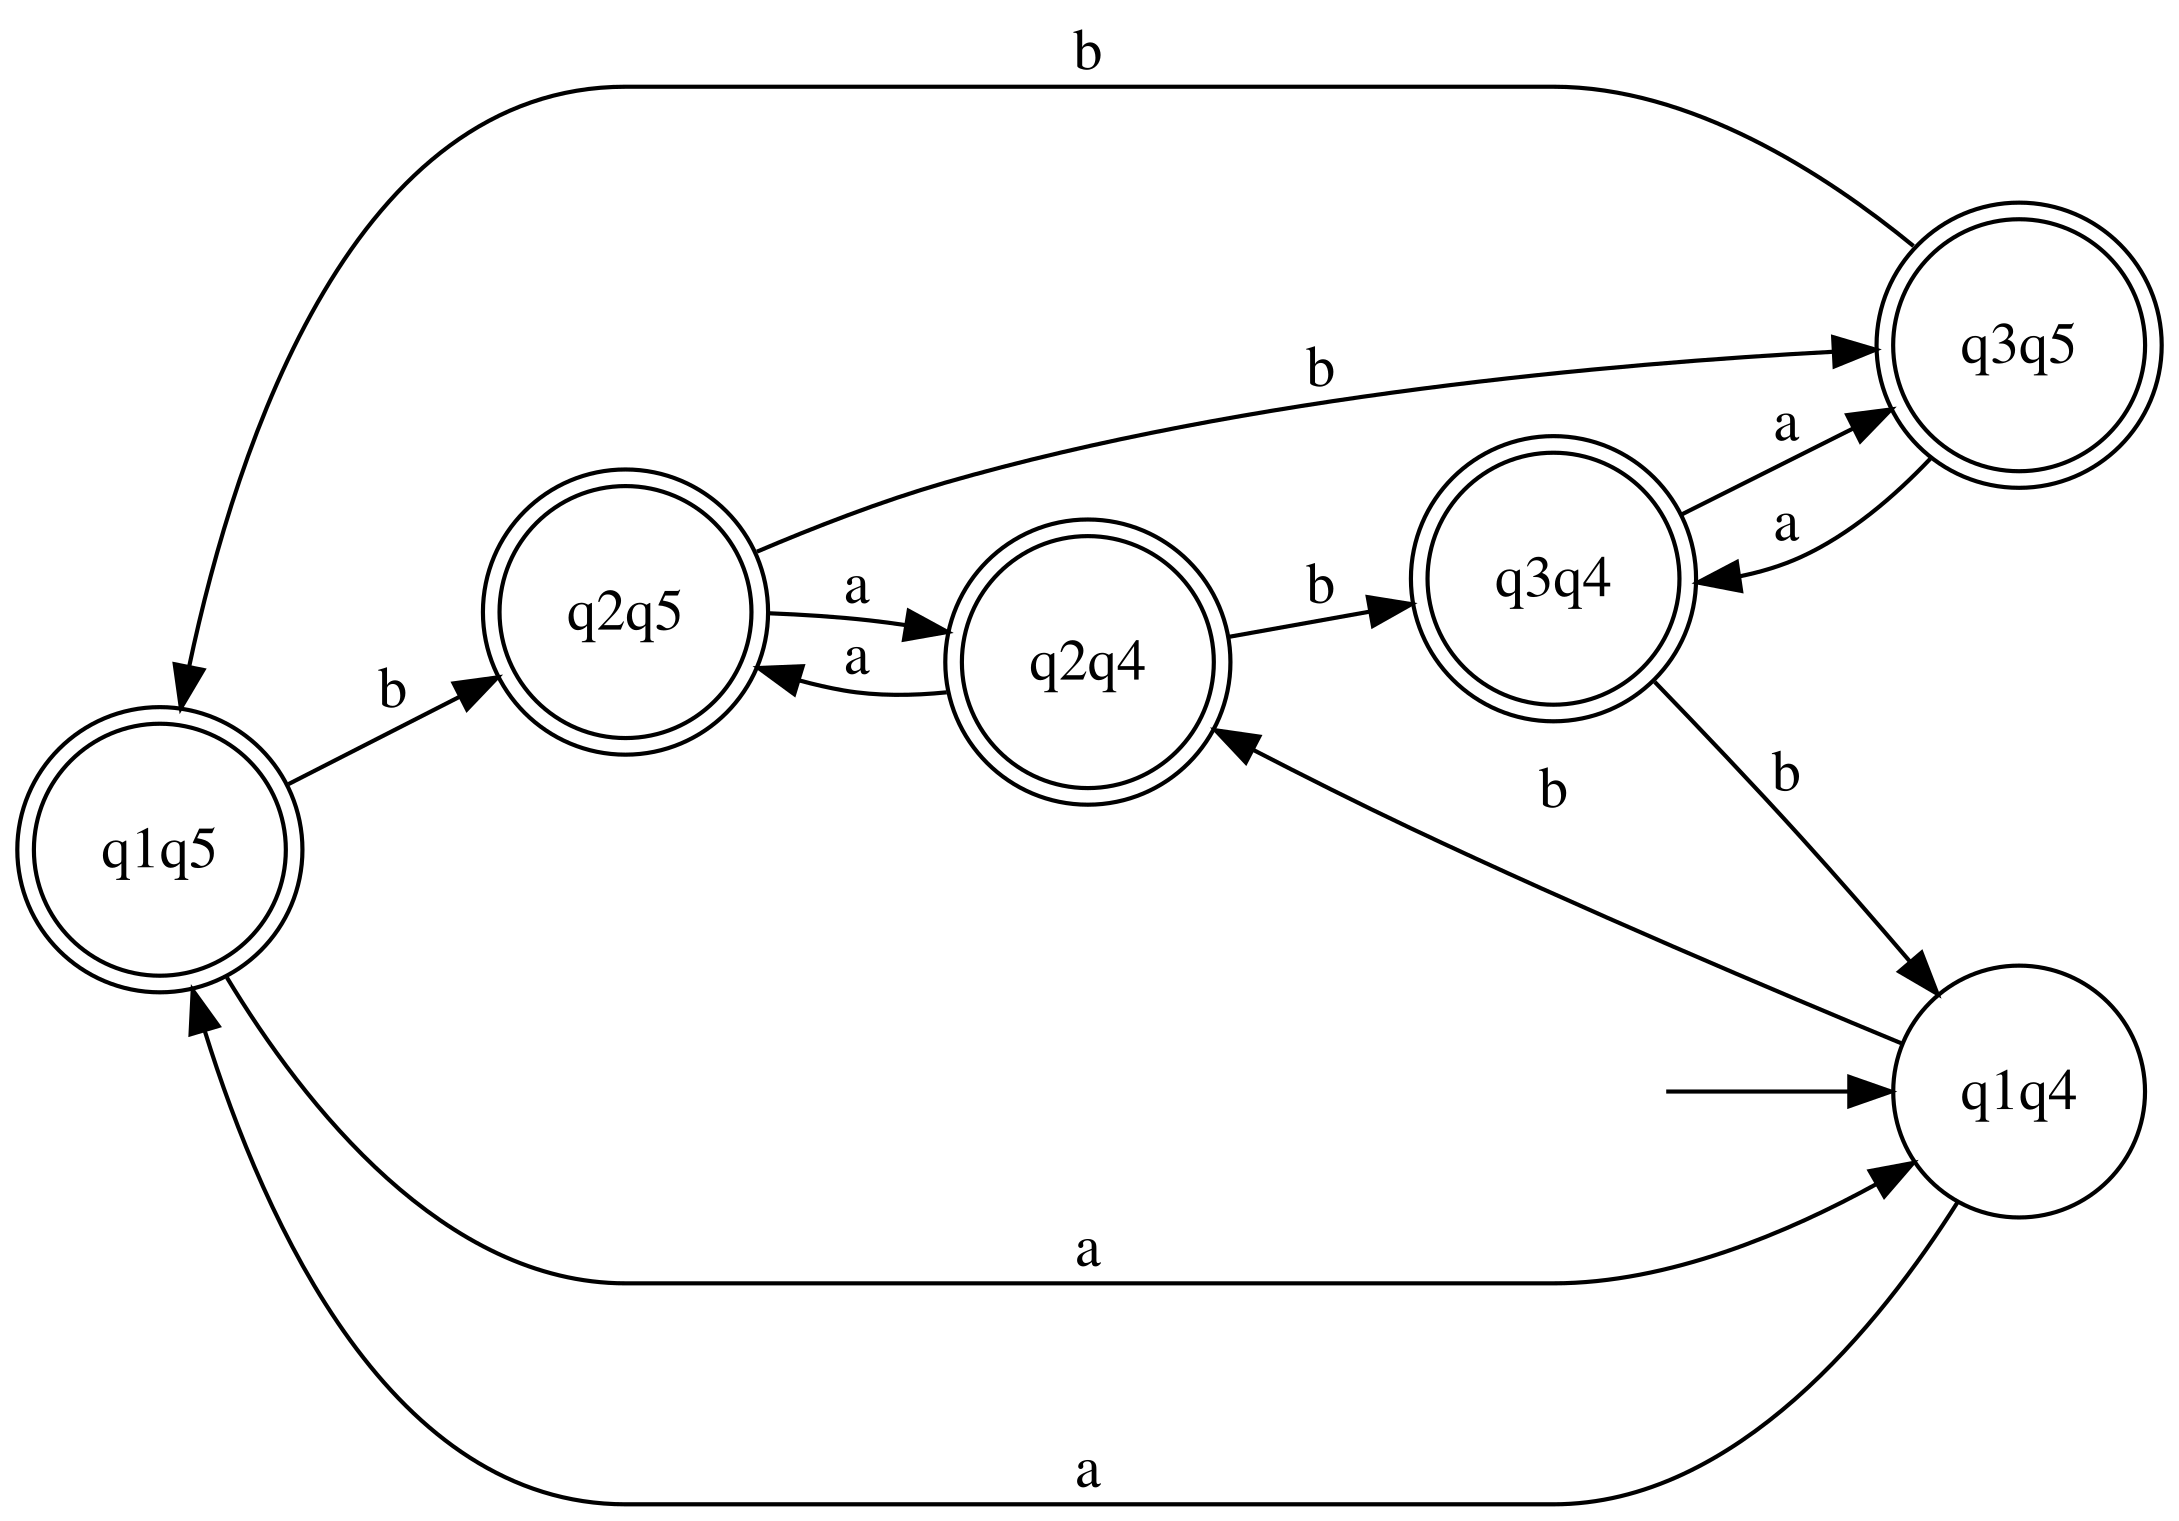
\includegraphics [scale=0.7]{2_4.png}\\\\
\\
2.5\\
L_5 = L_2/L_3\\
L_5 = L_2/L_3 = L_2 \cap \neg L_3\\
\textbf{За правильность не ручаюсь, но  вероятно все сделано правильно.}\\
\textbf{Выглядит страшно, но не ужасно}\\
\textbf{Часть узлов можно убрать, так как в них нельзя попасть, но я не стал этого делать}\\
\begin{tabular} {|c |c |c|}
\hline
 & a & b \\
\hline
\(q_1,q_1\) & \(q_2,g_4\) & \(q_2,g_2\) \\
\hline
\(q_1,q_2\) & \(q_2,g_5\) & \(q_2,g_3\) \\
\hline
\(q_1,q_3\) & \(q_2,g_6\) & \(q_2,g_1\) \\
\hline
\(q_1,q_4\) & \(q_2,g_1\) & \(q_2,g_5\) \\
\hline
\(q_1,q_5\) & \(q_2,g_2\) & \(q_2,g_6\) \\
\hline
\(q_1,q_6\) & \(q_2,g_3\) & \(q_2,g_4\) \\
\hline
\(q_2,q_1\) & \(q_3,g_4\) & \(q_3,g_2\) \\
\hline
\(q_2,q_2\) & \(q_3,g_5\) & \(q_3,g_3\) \\
\hline
\(q_2,q_3\) & \(q_3,g_6\) & \(q_3,g_1\) \\
\hline
\(q_2,q_4\) & \(q_3,g_1\) & \(q_3,g_5\) \\
\hline
\(q_2,q_5\) & \(q_3,g_2\) & \(q_3,g_6\) \\
\hline
\(q_2,q_6\) & \(q_3,g_3\) & \(q_3,g_4\) \\
\hline
\(q_3,q_1\) & \(q_4,g_4\) & \(q_3,g_2\) \\
\hline
\(q_3,q_2\) & \(q_4,g_5\) & \(q_3,g_3\) \\
\hline
\(q_3,q_3\) & \(q_4,g_6\) & \(q_3,g_1\) \\
\hline
\(q_3,q_4\) & \(q4,g_1\) & \(q_3,g_5\) \\
\hline
\(q_3,q_5\) & \(q_4,g_2\) & \(q_3,g_6\) \\
\hline
\(q_3,q_6\) & \(q_4,g_3\) & \(q_3,g_4\) \\
\hline
\(q_4,q_1\) & \(q_3,g_4\) & \(q_3,g_2\) \\
\hline
\(q_4,q_2\) & \(q_3,g_5\) & \(q_3,g_3\) \\
\hline
\(q_4,q_3\) & \(q_3,g_6\) & \(q_3,g_1\) \\
\hline
\(q_4,q_4\) & \(q_3,g_1\) & \(q_3,g_5\) \\
\hline
\(q_4,q_5\) & \(q_3,g_2\) & \(q_3,g_6\) \\
\hline
\(q_4,q_6\) & \(q_3,g_3\) & \(q_3,g_4\) \\
\hline
\hline
\end{tabular}\\
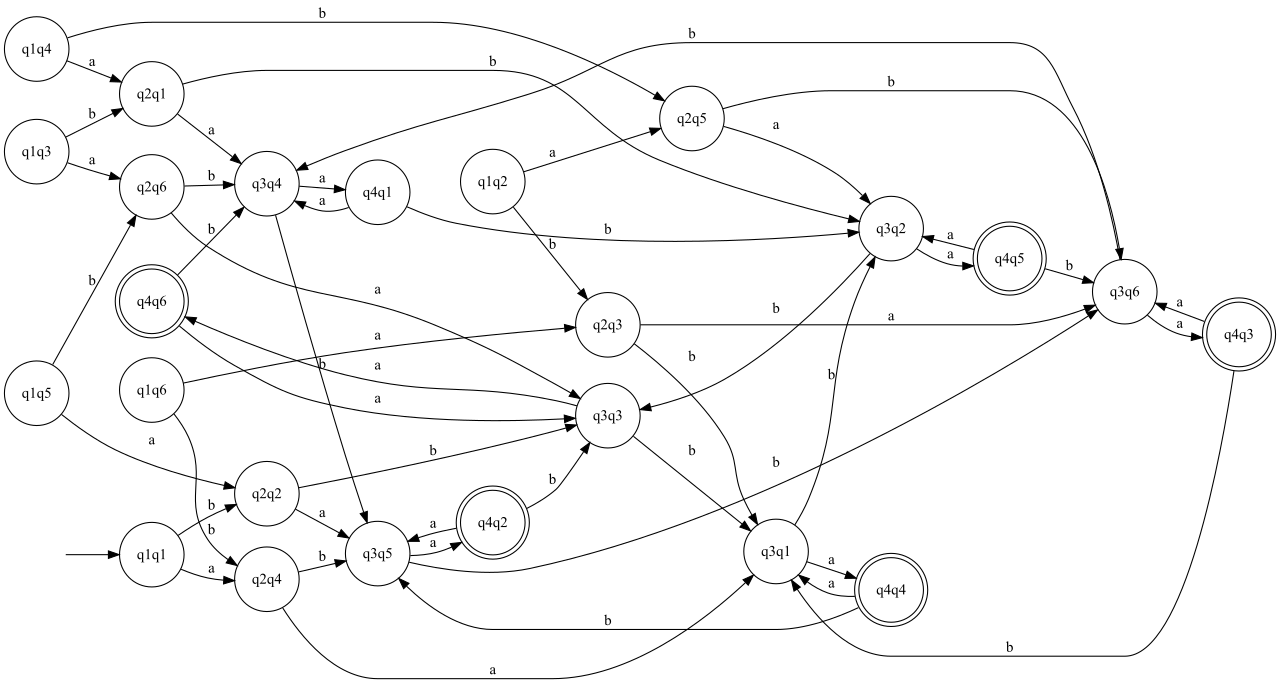
\includegraphics [scale=1]{2_5.png}\\\\
\\
\textbf{Задание 3. Построить минимальный ДКА по регулярному выражению}\\
3.1\\
(ab+aba)^*a\\
\text{НКА}\\
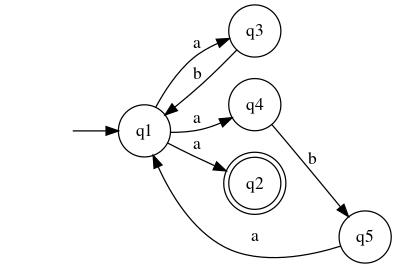
\includegraphics [scale=0.5]{3_1_НКА.png}\\
\text{Строим по алгоритму Томсона ДКА}\\
\begin{tabular} {|c |c |c|}
\hline
 & a & b \\
\hline
\(q_1\) & \(q_2,g_3,q_4\) & \(\) \\
\hline
\(q_2,g_3,q_4\) & \(\) & \(q_1,g_5\) \\
\hline
\(q_1,g_5\) & \(q_1,q_2,g_3,q_4\) & \(\) \\
\hline
\(q_1,q_2,g_3,q_4\) & \(q_2,g_3,q_4\) & \(q_1,g_5\) \\
\hline
\end{tabular}\\
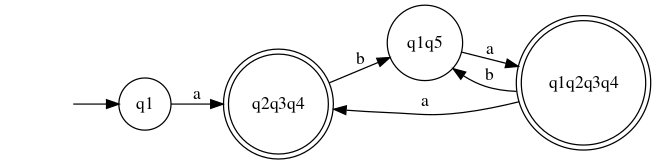
\includegraphics [scale=0.5]{3_1_ДКА.png}\\
\\
3.2\\
a(a(ab)^*b)^*(ab)^*\\
\text{НКА}\\
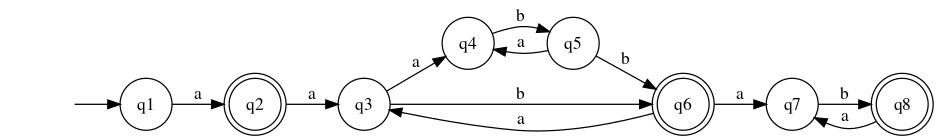
\includegraphics [scale=0.5]{3_2_НКА.png}\\
\text{Строим по алгоритму Томсона ДКА}\\
\begin{tabular} {|c |c |c|}
\hline
 & a & b \\
\hline
\(q_1\) & \(q_2\) & \(\) \\
\hline
\(q_2\) & \(q_3) & \(\) \\
\hline
\(q_3\) & \(q_4\) & \(q_6\) \\
\hline
\(q_4\) & \(\) & \(g_5\) \\
\hline
\(q_5\) & \(q_4\) & \(q_6\) \\
\hline
\(q_6\) & \(q_3,g_7\) & \(\) \\
\hline
\(q_3,q_7\) & \(q_4\) & \(q_6,g_8\) \\
\hline
\(q_6,q_8\) & \(q_3,g_7\) & \(\) \\
\hline
\end{tabular}\\
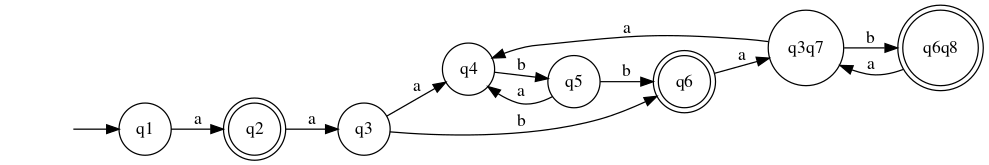
\includegraphics [scale=0.5]{3_2_ДКА.png}\\\
\begin{tabular} {|c |c |c |c |c |c |c |c |c |}
 & \(q_1\) & \(q_2\) & \(q_3\) & \(q_4\) & \(q_5\) & \(q_6\) & \(q_3q_7\) & \(q_6q_8\)\\
\hline
\(q_1\) & \(\) & \(+\) & \(+\) & \(+\) & \(+\) & \(+\) & \(+\) & \(+\) \\
\hline
\(q_2\) & \(+\) & \(\) & \(+\) & \(+\) & \(+\) & \(+\) & \(+\) & \(+\) \\
\hline
\(q_3\) & \(+\) & \(+\) & \(\) & \(+\) & \(+\) & \(+\) & \(\) & \(+\) \\
\hline
\(q_4\) & \(+\) & \(+\) & \(+\) & \(\) & \(+\) & \(+\) & \(+\) & \(+\) \\
\hline
\(q_5\) & \(+\) & \(+\) & \(+\) & \(+\) & \(\) & \(+\) & \(+\) & \(+\) \\
\hline
\(q_6\) & \(+\) & \(+\) & \(+\) & \(+\) & \(+\) & \(\) & \(+\) & \(\) \\
\hline
\(q_3,q_7\) & \(+\) & \(+\) & \(\) & \(+\) & \(+\) & \(+\) & \(\) & \(+\) \\
\hline
\(q_6,q_8\) & \(+\) & \(+\) & \(+\) & \(+\) & \(+\) & \(\) & \(+\) & \(\) \\
\hline
\end{tabular}\\
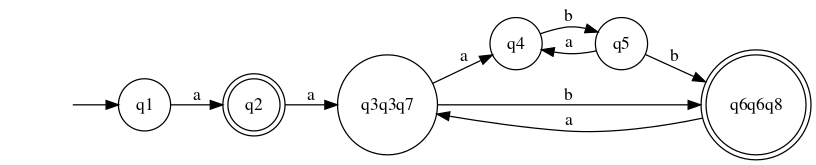
\includegraphics [scale=0.5]{3_2_МДКА.png}\\\
\\
3.3\\
(a+(a+b)(a+b)b)^*\\
\text{НКА}\\
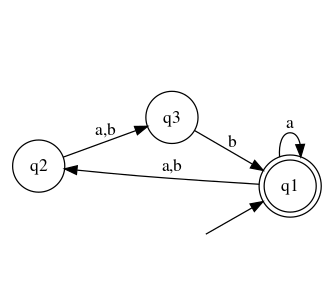
\includegraphics [scale=0.5]{3_3_НКА.png}\\
\text{Строим по алгоритму Томсона ДКА}\\
\begin{tabular} {|c |c |c|}
\hline
 & a & b \\
\hline
\(q_1\) & \(q_1,q_2\) & \(q_2\) \\
\hline
\(q_2\) & \(q_3) & \(q_3\) \\
\hline
\(q_3\) & \(\) & \(q_6\) \\
\hline
\(q_1,q_2\) & \(q_1,q_2,q_3\) & \(q_2,q_3\) \\
\hline
\(q_2,q_3\) & \(q_1,q_3\) & \(q_3\) \\
\hline
\(q_1,q_3\) & \(q_1,q_2\) & \(q_1,q_2\) \\
\hline
\(q_1,q_2,q_3\) & \(q_1,q_2,q_3\) & \(q_1,q_2,q_3\) \\
\hline

\end{tabular}\\
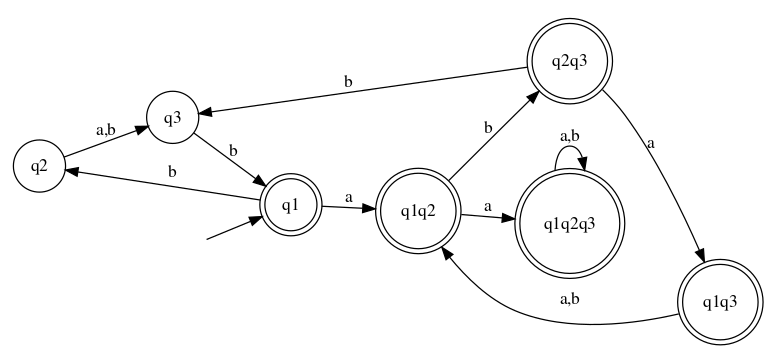
\includegraphics [scale=0.5]{3_3_ДКА.png}\\\
\\
3.4\\
(b+c)((ab)^*c+(ba)^*)^*\\
\text{НКА}\\
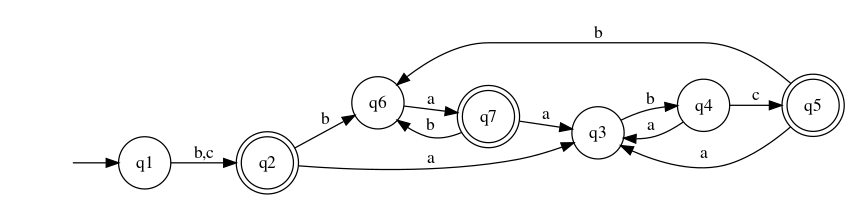
\includegraphics [scale=0.5]{3_4_НКА.png}\\
\text{Строим по алгоритму Томсона ДКА}\\
\begin{tabular} {|c |c |c| c|}
\hline
 & a & b & c\\
\hline
\(q_1\) & \(\) & \(q_2\) & \(q_2\) \\
\hline
\(q_2\) & \(q_3\) & \(q_6\) & \(\)  \\
\hline
\(q_3\) & \(\) & \(q_4\) & \(\)  \\
\hline
\(q_4\) & \(q_3\) & \(\) & \(q_5\)  \\
\hline
\(q_5\) & \(q_3\) & \(q_6\) & \(\)  \\
\hline
\(q_6\) & \(q_7\) & \(\) & \(\)  \\
\hline
\(q_7\) & \(q_3\) & \(q_6\) & \(\)  \\
\hline
\end{tabular}\\
\text{Получается ДКА представлен сверху}\\
\begin{tabular} {|c |c |c |c |c |c |c |c |}
 & \(q_1\) & \(q_2\) & \(q_3\) & \(q_4\) & \(q_5\) & \(q_6\) & \(q_7\) \\
\hline
\(q_1\) & \(\) & \(+\) & \(+\) & \(+\) & \(+\) & \(+\) & \(+\)  \\
\hline
\(q_2\) & \(+\) & \(\) & \(+\) & \(+\) & \(\) & \(+\) & \(\)  \\
\hline
\(q_3\) & \(+\) & \(+\) & \(\) & \(+\) & \(+\) & \(+\) & \(+\)  \\
\hline
\(q_4\) & \(+\) & \(+\) & \(+\) & \(\) & \(+\) & \(+\) & \(+\)  \\
\hline
\(q_5\) & \(+\) & \(\) & \(+\) & \(+\) & \(\) & \(+\) & \(\)  \\
\hline
\(q_6\) & \(+\) & \(+\) & \(+\) & \(+\) & \(+\) & \(\) & \(+\) \\
\hline
\(q_7\) & \(+\) & \(\) & \(+\) & \(+\) & \(\) & \(+\) & \(\) \\
\hline
\end{tabular}\\
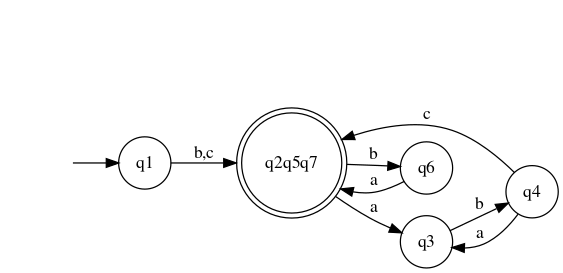
\includegraphics [scale=0.5]{3_4_МДКА.png}\\\
3.5\\
(a+b)^+(aa+bb+abab+baba)(a+b)^+\\
\text{НКА}\\
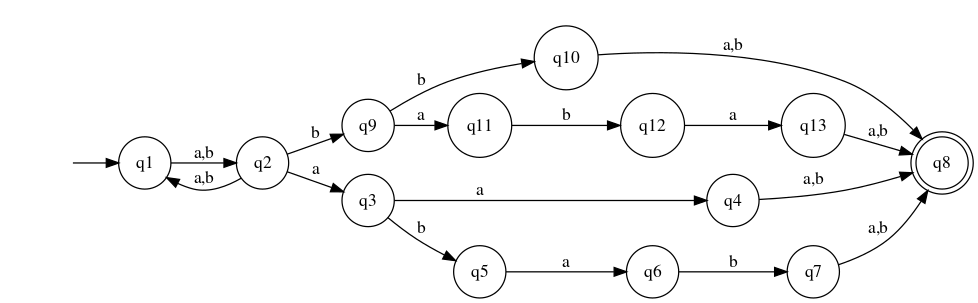
\includegraphics [scale=0.5]{3_5_НКА.png}\\
\\
\textbf{Задание 4. Определить является ли язык регулярным или нет}\\
4.1\\
L = \{(aab)^nb(aba)^m \mid n \geq 0 , m \geq 0\}\\\\
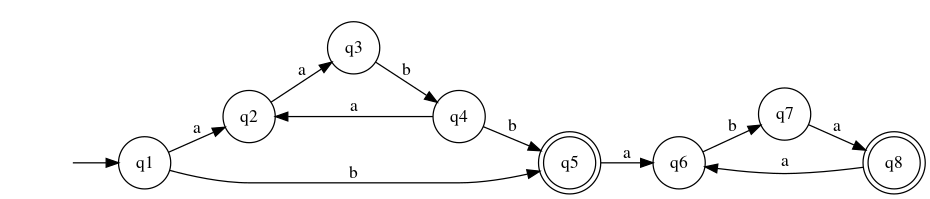
\includegraphics [scale=0.5]{4_1.png}\\
\text{Язык регулярный, так как понему можно построить ДКА}\\
\\
4.2\\
L = \{ uaav \mid u \in \{a,b\}^* , v \in a,b^*, |u|_b \geq |v|_a \}\\\\
\text{Рассмотрим слово }\\
w = b^naaa^n, \forall  n \in N, \text{ тогда } |w|=n+2+n>n \text{. Рассмотрим разбиения слова } w=xyz 
\text{ такие, что } |xy| \leq n, |y| \neq 0.\\
x=b^i,y=b^j, z=b^\(n-i-j\)aaa^n, 1 \leq i+j \leq n \text{ and } j>0\\
xy^0z=b^ib^\(n-i-j\)aaa^n=b^\(n-j\)aaa^n \notin L \implies \text{ L не регулярный язык}\\
\\
4.3\\
L = \{ a^mw \mid w \in \{a,b\}^* , 1 \leq |w|_b \leq m \}\\\\
\text{Рассмотрим слово }\\
w =a^n b^n, \forall  n \in N, \text{ тогда } |w|=n+n \geq n \text{. Рассмотрим разбиения слова } w=xyz 
\text{ такие, что } |xy| \leq n, |y| \neq 0.\\
x=a^i,y=a^j, z=a^\(n-i-j\)b^n, i+j \leq n \text{ and } j>0\\
xy^0z=a^ia^\(n-i-j\)b^n=a^\(n-j\)b^n \notin L \implies \text{ L не регулярный язык}\\
\\
4.4\\
L = \{ a^kb^ma^n \mid k = n \vee m > 0\}\\\\
\text{Рассмотрим слово }\\
w = a^nba^n, \forall  n \in N, \text{ тогда } |w|=n+1+n>n \text{. Рассмотрим разбиения слова } w=xyz 
\text{ такие, что } |xy| \leq n, |y| \neq 0.\\
x=a^i,y=a^j, z=a^\(n-i-j\)ba^n, i+j \leq n \text{ and } j>0\\
xy^2z=a^ia^\(2j\)a^\(n-i-j\)ba^n=a^\(n+j\)ba^n \notin L \implies \text{ L не регулярный язык.}\\
\text{На самом деле } y^2 \text{можно заменить на } y^m \text{ где } m \geq 2\\
\\
4.5\\
L = \{ ucv \mid u \in \{a,b\}^* , v \in \{a,b\}^*, u \neq v^R\}\\\\
\text{Рассмотрим слово }\\
w = (ab)^nc(ab)^n=\alpha_1\alpha_2...\alpha_\(4n+1\), \forall  n \in N, \text{ тогда } |w|=4n+1>n \text{. Рассмотрим разбиения слова } w=xyz 
\text{ такие, что } |xy| \leq n, |y| \neq 0.\\
x=\alpha_1\alpha_2...\alpha_\(i\),y=\alpha_\(i+1\)\alpha_\(i+2\)...\alpha_\(i+j\), z=\alpha_\(i+j+1\)\alpha_\(i+j+2\)...\alpha_\(4n+1\)c(ab)^n, i+j \leq n \text{ and } j>0\\
xy^2z=(\alpha_1\alpha_2...\alpha_\(i\))(\alpha_\(i+1\)\alpha_\(i+2\)...\alpha_\(i+j\))^2z
\notin L \implies \text{ L не регулярный язык.}\\
\text{В последней строчке добавил z, так как что-то произошло с латехом и он не хотел преобразовывавть формулу}\\
\\
\end{document}
